\chapter{System Description}\label{chap:systemDescribtion}
\textit{This chapter presents a description of the system configuration, which includes mechanical properties, sensors and actuators description and Attitude Determination and Control System (ADCS) approaches.}

The satellite used as a reference in this thesis is a CubeSat, depicted in figure \ref{fig:cube}, a pico-satellite that has been designed by California Polytechnic State University. This concept of satellite impose a few constrains. The dimensions of a 1U CubeSat  is $10 \times 10 \times 10 \ cm$ with a mass of 1kg, giving the advantage of having a light weight leading to a low power consumption, and a drawback of limited space. In order to enlarge the space within the satellite, the dimensions could be changed when designing it, such that a 3U design might be suitable for a satellite that will contain solar arrays or thrusters.

 From figure \ref{fig:cube} it can be seen that the satellite contains three magnetorquers shown as an example, but for the scope of the current thesis a pico-satellite equipped with three doubled and orthogonal magnetorquers is used. Also the CubeSat image shows the solar panels with on board electronics.

\begin{figure}[H]
	\centering
	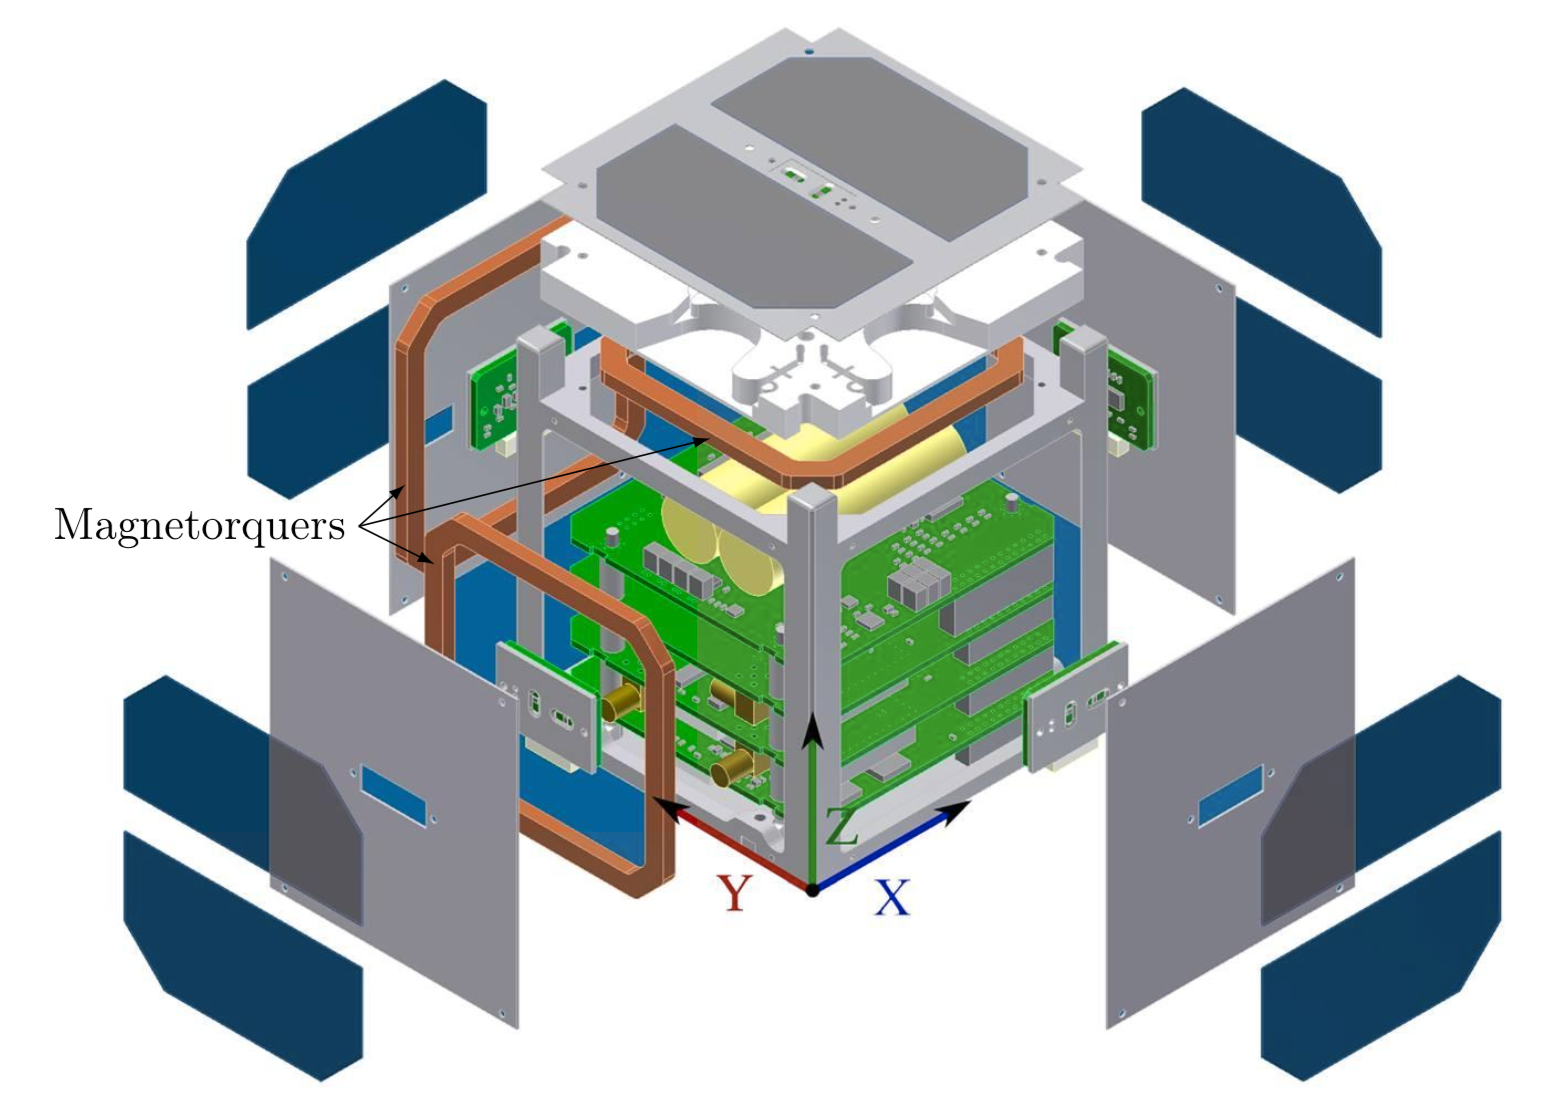
\includegraphics[width=0.7\linewidth]{figures/cubesat}
	\caption{CubeSat exploded view \cite{report}}
	\label{fig:cube}
\end{figure}

The satellite is equipped with two types of attitude actuators, magnetorquers and reaction wheeels. In order to keep the reaction wheels controllable, desaturation is performed using magnetorquers.

\subsubsection{ADCS approaches}
The objective of the ADCS system illustrated in figure \ref{fig:cubee} will be to control the angular velocity of the satellite and also to point to a specific target located on Earth. Therefore, a few procedures can be taken into account:

\textit{Detumbling} is the phase right after the satellite is deployed from the device called P-POD. The control goal during this phase is to decrease the angular velocity of the satellite.

\textit{Desaturation} means decreasing reaction wheel angular velocity in order to keep the wheels from saturation, thus keeping the wheels controllable in both directions.

\textit{Pointing} pointing involves keeping the satellite attitude stabilized at the reference attitude.


\begin{figure}[H]
	\centering
	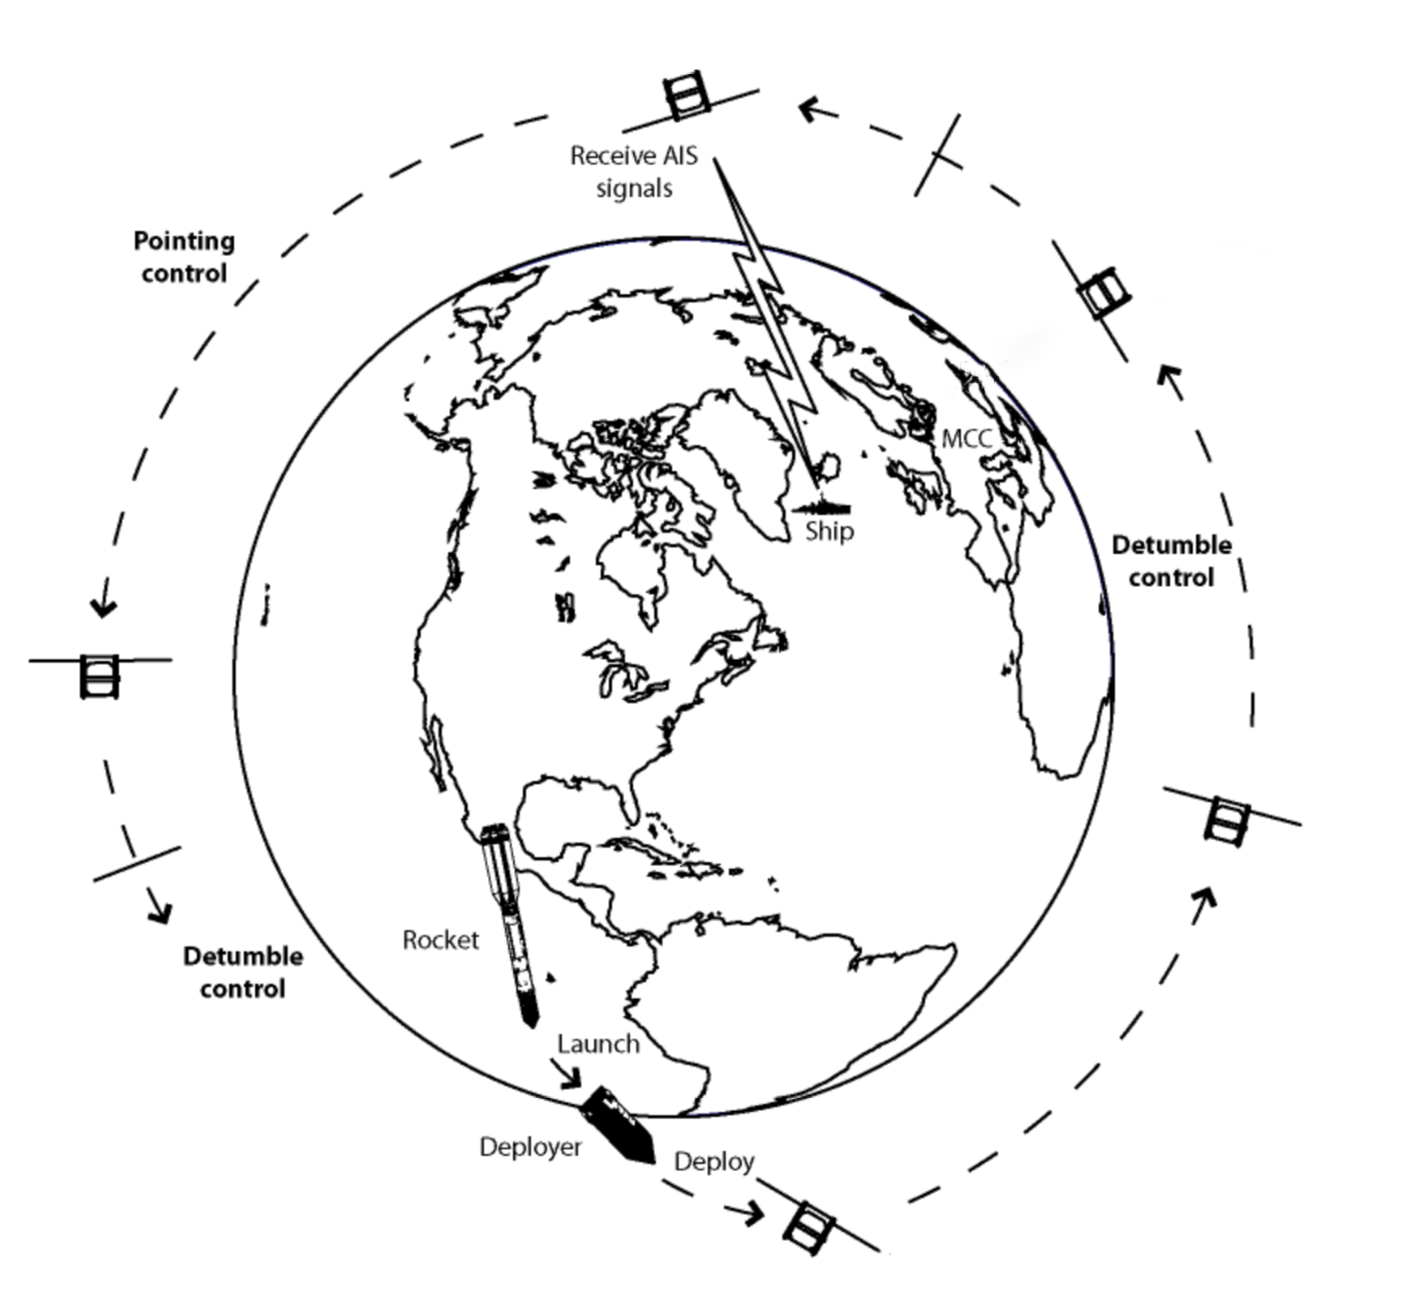
\includegraphics[width=0.7\linewidth]{figures/adcs}
	\caption{ADCS system description \cite{TH}}
	\label{fig:cubee}
\end{figure}

\nomenclature[AA]{\textbf{ADCS}}{Attitude Determination and Control System}

\section{Sensors}

\todo{describe the sensors}

\subsection{Magnetometer}

The orbit of the satellite is predictable, the satellite's location can be described as a function of time. Earth's magnetic field can also be quite accurately modeled. This means that by using magnetorquers, the orientation of the satellite can be approximated by comparing the magnetic field model at the satellite's current location and the direction of the magnetic field measured by the magnetometer. To address the noise in the measurement, including the noise arising from inside the satellite, Kalman or particle filtering, along with sensor fusion can be used, however this is outside of the scope of the thesis.

\subsection{Sun Tracking}

Sun trackers can be much easier to develop than star trackers. It measures the sun's orientation in relation to the satellite frame. By using it alongside other sensors, higher accuracy attitude estimation can be achieved, however when Earth is obstructing the sun rays, it is unable to provide attitude data, thus it is not sufficient to only use a sun tracking sensor.

\section{Actuators}
 This section describes the attitude actuators that the satellite is equipped with.
\subsection{Reaction Wheels}

One method of controlling a spacecraft's attitude is by using either reaction or momentum wheels attached to the spacecraft's body. The difference between momentum and reaction wheels is that the nominal angular velocity of momentum wheels is high in order to store angular momentum, while for reaction wheels, low. By controlling the wheel's angular velocity using a motor, the amount of angular momentum stored in the wheel can be controlled. If there are no external forces involved, the sum of angular momentum in the system made up by the spacecraft's body and the reaction wheels is constant. This means that by increasing the angular velocity of the wheels, the satellite body's angular momentum can be reduced. This angular momentum transfer can be used to control the attitude of the satellite. If the goal is to change the angular momentum of the whole satellite, actuators that are capable of external interaction should be used, such as magnetorquers or solar sails.

 In some satellites, the reaction wheels nominal speed is set higher than zero in order to avoid static friction in the bearings. Reaction wheels usually make up only a small fraction of a satellite's weight. They rely on being able to run at high speeds, making their angular momentum significant. The small weight ratio makes precise controlling easier.


%One design consideration for reaction wheels is maximizing moment of inertia for unit weight. This is done by distributing most of the material near the outskirts of the wheel. There is a trade-off between having most of the mass at the outskirts and durability at high angular velocities. 


Reaction wheels have an angular velocity limitation. This means that if a reaction wheel reaches its maximum angular velocity, it can no longer generate a torque on the satellite's body in one direction. In this scenario the system's controllability decreases, thus it should be avoided. An angular momentum unloading strategy should be designed to avoid it. Instead of returning the angular momentum to the satellite's body, unloading the angular momentum through other methods is preferred. Magnetorquers can be used for such purposes.

Moving parts are usually prone to failures. Reaction wheels are expected to occasionally run at high angular velocities, which wears down the lubrication and the bearings. Reaction wheels equipped with active magnetic bearings are in development \cite{MagneticReactWheel}. These can eliminate friction from the system and by controlling the bearing, can even reduce micro-vibrations, increasing the durability of the system. AAUSAT-II itself however uses mechanical wheel bearings.



\subsection{Magnetorquer}

Magnetorquers are special coils that can control the satellite's attitude by creating a magnetic momentum that interacts with Earth's magnetic field. It is capable of changing the total angular momentum of the satellite. Magnetorquers can only exert torque in two dimensions at any given moment, however over one orbit, three dimensional control can be achieved. In the investigated satellite they function as secondary actuators, with their purpose being the desaturation of the reaction wheels. Precise torque control can be achieved by setting up coaxial magnetorquers, one of which equipped with an iron core for larger magnetic field, the other lacking an iron core for finer magnetic field control.